\documentclass[12pt,a4paper]{article}

% ── Packages ──────────────────────────────────────────────
\usepackage[margin=1in]{geometry}
\usepackage{times}
\usepackage{setspace}
\usepackage{graphicx}
\usepackage{titlesec}
\usepackage{enumitem}
\usepackage{hyperref}
\usepackage{xcolor}
\usepackage{fancyhdr}
\usepackage{array}
\usepackage{longtable}
\usepackage{booktabs}
\usepackage{tikz}
\usepackage{float}
\usepackage{caption}
\usepackage{pgfplots}
\usepackage{tabularx}

\usetikzlibrary{shapes.geometric, arrows.meta, positioning, fit, calc, backgrounds}
\pgfplotsset{compat=1.18}

\hypersetup{
    colorlinks=true,
    linkcolor=blue!60!black,
    urlcolor=blue!70!black,
    citecolor=black,
}

% ── Spacing & Formatting ─────────────────────────────────
\onehalfspacing
\setlength{\parindent}{0pt}
\setlength{\parskip}{6pt}

\titleformat{\section}{\Large\bfseries}{\thesection.}{0.5em}{}[\vspace{2pt}\titlerule]
\titleformat{\subsection}{\large\bfseries}{\thesubsection}{0.5em}{}
\titleformat{\subsubsection}{\normalsize\bfseries}{\thesubsubsection}{0.5em}{}

% ── Header/Footer ────────────────────────────────────────
\pagestyle{fancy}
\fancyhf{}
\lhead{\small\textit{ScholarLens --- Software Requirements Specification}}
\rfoot{\thepage}
\renewcommand{\headrulewidth}{0.4pt}
\setlength{\headheight}{14pt}
\addtolength{\topmargin}{-2pt}

% ── TikZ styles ──────────────────────────────────────────
\tikzset{
    block/.style={
        rectangle, draw=blue!60!black, fill=blue!6,
        minimum width=3cm, minimum height=1cm,
        text centered, align=center, text width=2.5cm,
        rounded corners=3pt,
        font=\small\sffamily,
        line width=0.8pt,
    },
    bigblock/.style={
        rectangle, draw=teal!70!black, fill=teal!6,
        minimum width=4cm, minimum height=1.2cm,
        text centered, rounded corners=3pt,
        font=\small\sffamily\bfseries,
        line width=0.8pt,
    },
    infra/.style={
        rectangle, draw=orange!70!black, fill=orange!6,
        minimum width=3cm, minimum height=1cm,
        text centered, align=center, text width=2.5cm,
        rounded corners=3pt,
        font=\small\sffamily,
        line width=0.8pt,
    },
    user/.style={
        ellipse, draw=purple!60!black, fill=purple!6,
        minimum width=2cm, minimum height=1cm,
        text centered,
        font=\small\sffamily,
        line width=0.8pt,
    },
    arr/.style={
        -{Stealth[length=6pt]}, line width=0.7pt, color=gray!70!black
    },
    darr/.style={
        {Stealth[length=6pt]}-{Stealth[length=6pt]}, line width=0.7pt, color=gray!70!black
    },
    groupbox/.style={
        draw=gray!50, dashed, rounded corners=5pt, inner sep=10pt,
        fill=gray!3,
    },
}

% ══════════════════════════════════════════════════════════
\begin{document}

% ── Title Page ────────────────────────────────────────────
\begin{titlepage}
    \centering
    \vspace*{0.5cm}

    {\large\bfseries CHRIST (Deemed to be University), Bengaluru}\\[4pt]
    {\normalsize Department of Computer Science}\\[1.5cm]

    {\LARGE\bfseries Software Requirements Specification}\\[0.4cm]
    {\large Course: CSC481-5 --- Computer Science Project}\\[0.3cm]
    {\large Semester VI}\\[2cm]

    {\huge\bfseries ScholarLens}\\[0.3cm]
    {\Large Offline SLM-Based Research Literature Review Agent}\\[2.5cm]

    \begin{tabular}{l l l}
        \textbf{Sl. No.} & \textbf{Student Name} & \textbf{Register No.} \\[6pt]
        1. & Aditya Mehta   & 2440204 \\[4pt]
        2. & Jitvan Chadha  & 2440222 \\[4pt]
        3. & Ritesh K R     & 2440233 \\[4pt]
    \end{tabular}

    \vspace{2cm}

    \begin{tabular}{>{\bfseries}r l}
        Guide: & Dr. New Begin \\[4pt]
        Class: & 5BSC CS \\[4pt]
    \end{tabular}

    \vfill
    {\large June 2026}
\end{titlepage}

% ── Table of Contents ────────────────────────────────────
\tableofcontents
\newpage

% ══════════════════════════════════════════════════════════
%  SECTION 1 : Project Study
% ══════════════════════════════════════════════════════════
\section{Project Study}

\subsection{Introduction}
Research literature review is a fundamental step in academic and scientific
work.  Researchers and students routinely need to read, organise, and
synthesise large volumes of published papers to understand the current
state of knowledge in their field.  This process is predominantly
manual---time-consuming and prone to oversight, especially when dealing
with dozens of papers across related sub-topics.

Recent advances in language models have enabled AI-assisted literature
tools; however, these tools are cloud-dependent, raising concerns about
privacy, cost, and accessibility.  \textbf{ScholarLens} is proposed as a
fully offline, privacy-first research assistant that leverages locally
running Small Language Models (SLMs) to help researchers ingest, search,
analyse, and synthesise research papers---without any data leaving the
user's machine.

\subsection{Existing System}
Several tools exist in the research literature management space:

\begin{center}
\begin{tabularx}{\textwidth}{|l|X|l|}
    \hline
    \textbf{Tool} & \textbf{Description} & \textbf{Type} \\ \hline
    Zotero & Reference manager with PDF storage, annotation, and
              citation generation. & Offline/Sync \\ \hline
    Mendeley & Reference manager with social features and PDF
               reader. Owned by Elsevier. & Cloud-based \\ \hline
    Elicit & AI research assistant using LLMs to find and
             summarise papers. & Cloud (paid) \\ \hline
    Semantic Scholar & Academic search engine with AI-generated
                       TLDRs. & Cloud-based \\ \hline
    Connected Papers & Visualises citation graphs between papers. & Cloud-based \\ \hline
\end{tabularx}
\end{center}

\subsection{Limitations of the Existing System}
\begin{enumerate}[leftmargin=2em]
    \item \textbf{Internet dependency} --- Elicit, Semantic Scholar, and
          Connected Papers are entirely cloud-based and cannot be used
          offline.
    \item \textbf{Privacy concerns} --- Cloud tools require uploading
          research documents to third-party servers.
    \item \textbf{Limited analytical capability} --- Zotero and Mendeley
          are reference managers; they do not perform semantic search,
          summarisation, or gap analysis.
    \item \textbf{Cost} --- Advanced AI features in Elicit require paid
          subscriptions, limiting access for students.
    \item \textbf{No research gap identification} --- None of the
          existing tools automatically identify under-explored areas
          across a user's paper collection.
\end{enumerate}

\subsection{Proposed System}
ScholarLens is a self-contained, offline web application that provides:
\begin{itemize}[leftmargin=2em]
    \item PDF ingestion with automatic text extraction, chunking, and
          metadata parsing.
    \item Hybrid search combining semantic embeddings with BM25
          keyword matching.
    \item SLM-powered analysis: summarisation, claim extraction, and
          thematic clustering.
    \item Automated research gap identification with suggested future
          directions.
    \item A browser-based interface requiring no additional software
          beyond the runtime.
\end{itemize}

\subsection{Benefits of the Proposed System}
\begin{enumerate}[leftmargin=2em]
    \item \textbf{Complete privacy} --- All processing occurs locally;
          no data is transmitted externally.
    \item \textbf{Zero recurring cost} --- Uses open-source models and
          tools with no subscriptions or API fees.
    \item \textbf{Offline operation} --- Fully functional without internet
          after initial setup.
    \item \textbf{Comprehensive analysis} --- Goes beyond reference
          management to deliver actionable research insights.
    \item \textbf{Modular and extensible} --- New capabilities can be
          added independently without disrupting existing functionality.
\end{enumerate}

\newpage

% ══════════════════════════════════════════════════════════
%  SECTION 2 : Literature Survey
% ══════════════════════════════════════════════════════════
\section{Literature Survey}

\subsection{Transformer-Based Language Models}
The transformer architecture (Vaswani et al., 2017) has fundamentally
changed NLP.  BERT (Devlin et al., 2019) introduced bidirectional
pre-training for strong performance on comprehension tasks.  The LLaMA
family (Touvron et al., 2023) subsequently showed that smaller open models
(1B--8B parameters) can achieve competitive results on consumer hardware.
Frameworks like \textbf{Ollama} now allow users to run these models locally
with a simple command-line interface.

\subsection{Sentence Embeddings and Semantic Search}
Sentence-BERT (Reimers \& Gurevych, 2019) fine-tunes BERT-like models to
produce semantically meaningful sentence-level embeddings.  The
\texttt{all-MiniLM-L6-v2} variant offers an effective trade-off between
quality and speed, producing 384-dimensional vectors suitable for cosine
similarity search.

\subsection{Retrieval-Augmented Generation}
Lewis et al.\ (2020) proposed RAG, which combines a retrieval component
with a generative model.  Instead of relying solely on the LLM's parametric
knowledge, relevant documents are retrieved and provided as context,
reducing hallucination and grounding outputs in source material.

\subsection{BM25 and Hybrid Retrieval}
BM25 (Robertson \& Zaragoza, 2009) remains a strong keyword retrieval
baseline.  Recent work shows that hybrid approaches---combining dense
semantic embeddings with sparse BM25 scores---consistently outperform
either method alone (Karpukhin et al., 2020).

\subsection{Vector Databases}
Vector databases such as ChromaDB and FAISS are optimised for approximate
nearest-neighbour search over high-dimensional embeddings.  ChromaDB is
chosen for this project due to its lightweight, Python-native API and
persistent file-based storage.

\vspace{6pt}
\textbf{References:}
\begin{enumerate}[leftmargin=2em, label={[\arabic*]}]
    \item Vaswani, A. et al., ``Attention Is All You Need,''
          \textit{NeurIPS}, 2017.
    \item Devlin, J. et al., ``BERT: Pre-training of Deep Bidirectional
          Transformers,'' \textit{NAACL-HLT}, 2019.
    \item Touvron, H. et al., ``LLaMA: Open and Efficient Foundation
          Language Models,'' \textit{arXiv:2302.13971}, 2023.
    \item Reimers, N. and Gurevych, I., ``Sentence-BERT,''
          \textit{EMNLP}, 2019.
    \item Lewis, P. et al., ``Retrieval-Augmented Generation for
          Knowledge-Intensive NLP Tasks,'' \textit{NeurIPS}, 2020.
    \item Robertson, S. and Zaragoza, H., ``The Probabilistic Relevance
          Framework: BM25 and Beyond,'' \textit{FnT in IR}, 2009.
    \item Karpukhin, V. et al., ``Dense Passage Retrieval for Open-Domain
          QA,'' \textit{EMNLP}, 2020.
\end{enumerate}

\newpage

% ══════════════════════════════════════════════════════════
%  SECTION 3 : Requirements Specification
% ══════════════════════════════════════════════════════════
\section{Requirements Specification}

\subsection{Functional Requirements}

\begin{longtable}{|c|p{3.5cm}|p{7.5cm}|}
    \hline
    \textbf{ID} & \textbf{Requirement} & \textbf{Description} \\ \hline
    \endfirsthead
    \hline
    \textbf{ID} & \textbf{Requirement} & \textbf{Description} \\ \hline
    \endhead
    \hline
    \endfoot

    FR-01 & PDF Upload &
    The system shall allow users to upload research papers in PDF format
    via a web interface. \\ \hline

    FR-02 & Text Extraction &
    The system shall extract text from uploaded PDFs, handling
    multi-column layouts. \\ \hline

    FR-03 & Metadata Extraction &
    The system shall extract metadata (title, authors, abstract, year)
    from papers where available. \\ \hline

    FR-04 & Text Chunking &
    The system shall segment text into configurable chunks with overlap
    to preserve context. \\ \hline

    FR-05 & Embedding Generation &
    The system shall generate vector embeddings for each chunk using a
    local embedding model. \\ \hline

    FR-06 & Vector Storage &
    The system shall persist embeddings in a local vector database. \\ \hline

    FR-07 & Semantic Search &
    The system shall perform similarity search over embeddings given a
    natural language query. \\ \hline

    FR-08 & Keyword Search &
    The system shall support BM25-based keyword search. \\ \hline

    FR-09 & Hybrid Search &
    The system shall combine semantic and keyword search results using
    score fusion. \\ \hline

    FR-10 & Summarisation &
    The system shall generate summaries of selected papers using a
    local SLM. \\ \hline

    FR-11 & Claim Extraction &
    The system shall extract key claims and findings from papers. \\ \hline

    FR-12 & Theme Clustering &
    The system shall group papers by thematic similarity. \\ \hline

    FR-13 & Gap Analysis &
    The system shall identify under-explored areas across the user's
    paper collection. \\ \hline

    FR-14 & Direction Suggestions &
    The system shall suggest potential research directions based on
    identified gaps. \\ \hline

    FR-15 & Library Management &
    The system shall allow users to browse, view, and delete ingested
    papers. \\ \hline

    FR-16 & Health Check &
    The system shall verify that all backend services are operational. \\ \hline
\end{longtable}

\textbf{Exceptional behaviour:} If the Ollama model server is not running,
the system shall display a clear error message indicating the service is
unavailable and disable analysis features. Corrupt or unsupported PDF files
shall be rejected with an appropriate error. Search on an empty knowledge
base shall return an informative empty-state message.

\subsection{Non-Functional Requirements}

\begin{longtable}{|c|p{3.5cm}|p{8cm}|}
    \hline
    \textbf{ID} & \textbf{Requirement} & \textbf{Description} \\ \hline
    \endfirsthead
    \hline
    \textbf{ID} & \textbf{Requirement} & \textbf{Description} \\ \hline
    \endhead
    \hline
    \endfoot

    NFR-01 & Offline Operation &
    The system shall work entirely offline after initial setup. \\ \hline

    NFR-02 & Privacy &
    No user data shall be sent to any external server. \\ \hline

    NFR-03 & Performance &
    Search queries shall return within 3 seconds for up to 100
    papers. \\ \hline

    NFR-04 & Usability &
    The interface shall be intuitive and require no technical
    training. \\ \hline

    NFR-05 & Portability &
    The system shall run on Windows, macOS, and Linux. \\ \hline

    NFR-06 & Configurability &
    Key parameters (model, chunk size, top-K) shall be configurable
    via environment variables. \\ \hline
\end{longtable}

\subsection{Software Requirements}

\begin{center}
\begin{tabularx}{\textwidth}{|l|X|}
    \hline
    \textbf{Software} & \textbf{Specification} \\ \hline
    Operating System & Windows 10/11, macOS 12+, or Ubuntu 20.04+ \\ \hline
    Python & 3.11 or higher \\ \hline
    Node.js & 18 or higher \\ \hline
    Ollama & Latest stable release with a pulled SLM (e.g.\ LLaMA 3.2) \\ \hline
    Web Browser & Chrome, Firefox, Edge, or Safari \\ \hline
\end{tabularx}
\end{center}

\subsection{Hardware Requirements}

\begin{center}
\begin{tabularx}{\textwidth}{|l|X|X|}
    \hline
    \textbf{Component} & \textbf{Minimum} & \textbf{Recommended} \\ \hline
    Processor & Quad-core x86\_64 & 8-core / Apple M-series \\ \hline
    RAM & 8 GB & 16 GB \\ \hline
    Storage & 10 GB free & 20 GB (SSD preferred) \\ \hline
    GPU & Not required & NVIDIA 6 GB+ VRAM \\ \hline
\end{tabularx}
\end{center}



% ══════════════════════════════════════════════════════════
%  SECTION 4 : System Models
% ══════════════════════════════════════════════════════════
\section{System Models}

\subsection{System Architecture (Block Diagram)}

\begin{figure}[H]
\centering
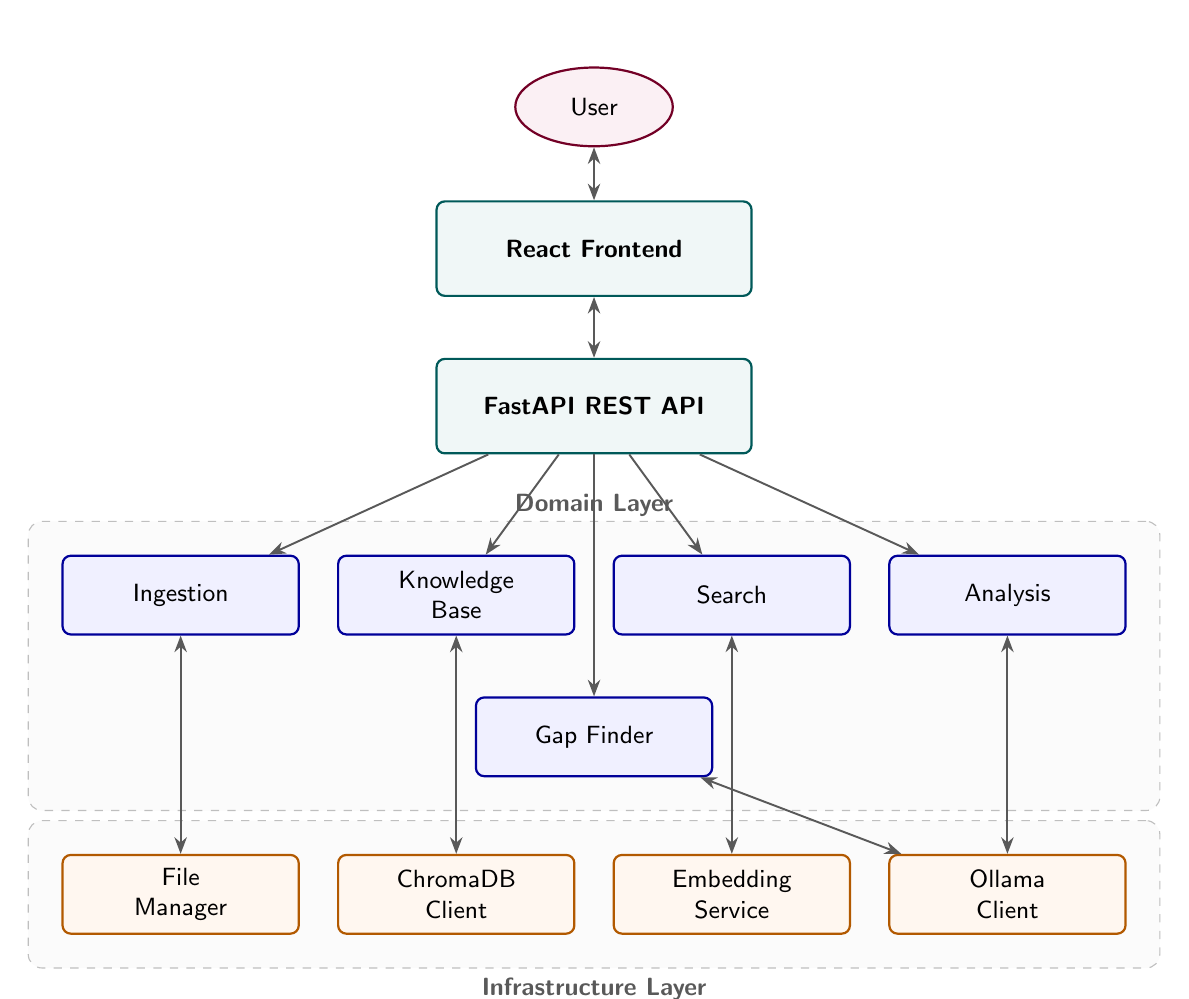
\begin{tikzpicture}

    % ── User ──
    \node[user] (user) at (0, 0) {User};

    % ── Frontend ──
    \node[bigblock] (frontend) at (0, -1.8) {React Frontend};

    % ── API Layer ──
    \node[bigblock] (api) at (0, -3.8) {FastAPI REST API};

    % ── Domain modules row 1 (4 modules, 3.5cm spacing) ──
    \node[block] (ingest)   at (-5.25, -6.2) {Ingestion};
    \node[block] (kb)       at (-1.75, -6.2) {Knowledge\\Base};
    \node[block] (search)   at (1.75, -6.2)  {Search};
    \node[block] (analysis) at (5.25, -6.2)  {Analysis};

    % ── Domain module row 2 (centered) ──
    \node[block] (gap) at (0, -8.0) {Gap Finder};

    % ── Infrastructure (aligned under row 1 domain nodes) ──
    \node[infra] (files)  at (-5.25, -10.0) {File\\Manager};
    \node[infra] (chroma) at (-1.75, -10.0) {ChromaDB\\Client};
    \node[infra] (embed)  at (1.75, -10.0)  {Embedding\\Service};
    \node[infra] (ollama) at (5.25, -10.0)  {Ollama\\Client};

    % ── Arrows: User <-> Frontend <-> API ──
    \draw[darr] (user)     -- (frontend);
    \draw[darr] (frontend) -- (api);

    % ── Arrows: API -> Domain row 1 ──
    \draw[arr] (api) -- (ingest);
    \draw[arr] (api) -- (kb);
    \draw[arr] (api) -- (search);
    \draw[arr] (api) -- (analysis);

    % ── Arrow: API -> Gap Finder ──
    \draw[arr] (api) -- (gap);

    % ── Arrows: Domain <-> Infrastructure ──
    \draw[darr] (ingest)   -- (files);
    \draw[darr] (kb)       -- (chroma);
    \draw[darr] (search)   -- (embed);
    \draw[darr] (analysis) -- (ollama);
    \draw[darr] (gap) -- (ollama);

    % ── Group boxes ──
    \begin{scope}[on background layer]
        \node[groupbox,
              fit=(ingest)(kb)(search)(analysis)(gap),
              inner sep=12pt,
              label={[font=\small\sffamily\bfseries,
                      text=gray!70!black, yshift=-2pt]above:Domain Layer}] {};
        \node[groupbox,
              fit=(files)(chroma)(embed)(ollama),
              inner sep=12pt,
              label={[font=\small\sffamily\bfseries,
                      text=gray!70!black]below:Infrastructure Layer}] {};
    \end{scope}

\end{tikzpicture}
\caption{High-Level System Architecture of ScholarLens}
\label{fig:architecture}
\end{figure}

\newpage

\subsection{Module Descriptions}

\subsubsection{Module 1: Document Ingestion}

Handles the intake of raw PDF files and converts them into structured text.
\begin{itemize}[leftmargin=2em]
    \item \textbf{PDF Parser} --- Extracts text from PDF files using PyMuPDF
          with pdfplumber as fallback for complex layouts.
    \item \textbf{Text Chunker} --- Splits text into fixed-size chunks
          (default 512 tokens, 50-token overlap) respecting sentence
          boundaries.
    \item \textbf{Metadata Extractor} --- Parses PDF metadata and uses
          heuristics to identify title, authors, abstract, and year.
\end{itemize}

\subsubsection{Module 2: Knowledge Base}

Manages persistent storage and retrieval of document embeddings.
\begin{itemize}[leftmargin=2em]
    \item \textbf{Embedding Service} --- Generates 384-dim vectors using
          the \texttt{all-MiniLM-L6-v2} sentence-transformer model.
    \item \textbf{Repository} --- CRUD operations on ChromaDB for storing
          and querying chunks with their embeddings.
\end{itemize}

\subsubsection{Module 3: Search \& Retrieval}

Provides intelligent passage retrieval from the knowledge base.
\begin{itemize}[leftmargin=2em]
    \item \textbf{Semantic Search} --- Cosine similarity over dense
          embeddings.
    \item \textbf{Keyword Search} --- BM25 ranking over the text corpus.
    \item \textbf{Hybrid Search} --- Fuses semantic and keyword scores
          to return top-K results.
\end{itemize}

\subsubsection{Module 4: Analysis}

Uses the local SLM for higher-order text analysis.
\begin{itemize}[leftmargin=2em]
    \item \textbf{Summariser} --- Generates concise paper summaries by
          providing retrieved chunks as context to the SLM.
    \item \textbf{Claim Extractor} --- Identifies key findings using
          structured prompting.
    \item \textbf{Theme Clusterer} --- Groups papers by topic similarity.
\end{itemize}

\subsubsection{Module 5: Gap Finder}

Analyses the full paper collection for under-explored areas.
\begin{itemize}[leftmargin=2em]
    \item \textbf{Gap Analyser} --- Identifies thin, contradictory, or
          absent coverage areas.
    \item \textbf{Suggestion Engine} --- Generates research direction
          suggestions grounded in the user's papers.
\end{itemize}

\subsubsection{Module 6: Infrastructure}

Adapters isolating domain logic from external services.
\begin{itemize}[leftmargin=2em]
    \item \textbf{Ollama Client} --- HTTP client for local SLM inference,
          model listing, and health checks.
    \item \textbf{ChromaDB Client} --- Manages vector store connection and
          collection lifecycle.
    \item \textbf{File Manager} --- Filesystem operations for PDF storage
          and directory management.
\end{itemize}

\subsubsection{Module 7: API Layer}

Exposes domain functionality as RESTful endpoints:

\begin{center}
\begin{tabularx}{\textwidth}{|l|l|X|}
    \hline
    \textbf{Method} & \textbf{Endpoint} & \textbf{Function} \\ \hline
    POST   & /api/documents/upload   & Upload and ingest a PDF \\ \hline
    GET    & /api/documents          & List all papers \\ \hline
    GET    & /api/documents/\{id\}   & Get paper details \\ \hline
    DELETE & /api/documents/\{id\}   & Delete a paper \\ \hline
    POST   & /api/search             & Hybrid search \\ \hline
    POST   & /api/analysis/summarize & Generate summaries \\ \hline
    POST   & /api/analysis/claims    & Extract claims \\ \hline
    POST   & /api/analysis/themes    & Cluster by themes \\ \hline
    POST   & /api/gaps/analyze       & Gap analysis \\ \hline
    GET    & /api/system/health      & Health check \\ \hline
    GET    & /api/system/models      & List Ollama models \\ \hline
    GET    & /api/system/stats       & KB statistics \\ \hline
\end{tabularx}
\end{center}

\subsubsection{Module 8: Frontend}

Browser-based React SPA with five views:
\begin{itemize}[leftmargin=2em]
    \item \textbf{Upload Panel} --- Drag-and-drop PDF upload.
    \item \textbf{Library} --- Browse and manage ingested papers.
    \item \textbf{Search} --- Query input with ranked passage results.
    \item \textbf{Analysis} --- Trigger summarisation, claim extraction,
          and theme clustering.
    \item \textbf{Gap Analysis} --- View research gaps and suggestions.
\end{itemize}

\end{document}
